\section{Localització dels punts a l'espai}

Per localitzar punts a l'espai tridimensional s'utilitza un \textbf{sistema de referència cartesià} format per tres rectes perpendiculars entre si que s'anomenen \textbf{eixos de coordenades}, designats per $x$, $y$ i $z$. Qualsevol punt de l'espai queda determinat per tres coordenades $(x, y, z)$.

\begin{figure}[H]
\centering
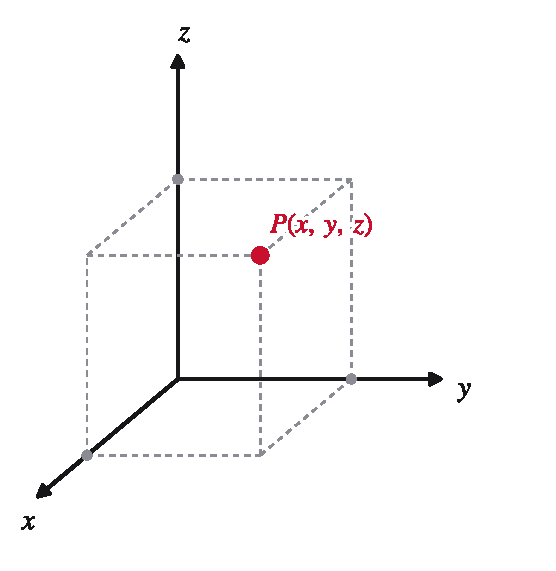
\includegraphics[width=267pt]{fig/m06_f14.pdf}
\caption{Sistema de coordenades cartesianes a l'espai: qualsevol punt $P$ queda determinat per la terna $(x, y, z)$.}
\end{figure}

\section{Components d'un vector a l'espai}

\textbf{Definició:} Els \textbf{components} d'un vector s'obtenen restant ordenadament les coordenades del seu extrem menys les del seu origen. Donats els punts $A(a_1, a_2, a_3)$ i $B(b_1, b_2, b_3)$, el vector $\overrightarrow{AB}$ té components:

\begin{equation}
\overrightarrow{AB} = (b_1 - a_1,\; b_2 - a_2,\; b_3 - a_3)
\end{equation}

Per definir un vector calen tres elements: \textbf{direcció}, \textbf{sentit} i \textbf{magnitud} (mòdul).

Si el vector $\overrightarrow{AB}$ té la mateixa longitud, direcció i sentit que un altre vector $\overrightarrow{CD}$, es tracta de dos vectors \textbf{equipol\textperiodcentered{}lents}. El conjunt de tots els vectors fixos equipol\textperiodcentered{}lents s'anomena \textbf{vector lliure}.

\subsection{Mòdul d'un vector}

El mòdul d'un vector $\vec v = (v_1, v_2, v_3)$ és la seva longitud:

\begin{equation*}
|\vec v| = \sqrt{v_1^2 + v_2^2 + v_3^2}
\end{equation*}

\subsection{Vector unitari}

El vector unitari en la direcció de $\vec v$ és aquell de mòdul 1:

\begin{equation*}
\hat u_v = \frac{\vec v}{|\vec v|}
\end{equation*}

\section{Operacions amb vectors}

\subsection{Suma de vectors}

Donats $\vec a = (a_1, a_2, a_3)$ i $\vec b = (b_1, b_2, b_3)$, el seu vector suma és:

\begin{equation*}
\vec a + \vec b = (a_1 + b_1,\; a_2 + b_2,\; a_3 + b_3)
\end{equation*}

La suma de vectors compleix les propietats següents:

\begin{itemize}
\item \textbf{Commutativa:} $\vec a + \vec b = \vec b + \vec a$
\item \textbf{Associativa:} $\vec a + (\vec b + \vec c) = (\vec a + \vec b) + \vec c$
\item \textbf{Element neutre:} el vector nul $\vec 0 = (0, 0, 0)$ compleix $\vec a + \vec 0 = \vec a$
\item \textbf{Element simètric:} cada vector $\vec a$ té un oposat $-\vec a$ tal que $\vec a + (-\vec a) = \vec 0$
\end{itemize}

\subsection{Multiplicació d'un vector per un escalar}

Donat $k \in \mathbb{R}$ i $\vec a = (a_1, a_2, a_3)$:

\begin{equation*}
k\cdot\vec a = (k a_1,\; k a_2,\; k a_3)
\end{equation*}

Propietats:

\begin{itemize}
\item $k\cdot(\vec a + \vec b) = k\vec a + k\vec b$
\item $1\cdot\vec a = \vec a$
\item $(k + h)\cdot\vec a = k\vec a + h\vec a$
\item $(k\cdot h)\cdot\vec a = k\,(h\cdot\vec a)$
\end{itemize}

\section{Combinació lineal de vectors}

\textbf{Definició:} Donat un conjunt de vectors $\vec v_1, \vec v_2, \vec v_3$ d'un espai vectorial, s'anomena \textbf{combinació lineal} d'aquests vectors tota expressió de la forma

\begin{equation}
\lambda_1\vec v_1 + \lambda_2\vec v_2 + \lambda_3\vec v_3 + \cdots
\end{equation}

on $\lambda_1, \lambda_2, \lambda_3, \ldots \in \mathbb{R}$.

Un vector $\vec v$ és combinació lineal de $\vec v_1, \vec v_2, \vec v_3$ si existeixen $\lambda_1, \lambda_2, \lambda_3$ que verifiquen l'expressió anterior.

\section{Dependència i independència lineal de vectors}

Els vectors $\vec v_1, \vec v_2, \vec v_3$ són \textbf{linealment independents} si l'única solució de

\begin{equation*}
\lambda_1\vec v_1 + \lambda_2\vec v_2 + \lambda_3\vec v_3 = \vec 0
\end{equation*}

és $\lambda_1 = \lambda_2 = \lambda_3 = 0$. En cas contrari, és a dir, si existeix alguna solució amb algun $\lambda_i \neq 0$, els vectors són \textbf{linealment dependents} (un d'ells és combinació lineal dels altres).

\section{Producte escalar de dos vectors}

\textbf{Definició:} El \textbf{producte escalar} de dos vectors $\vec a$ i $\vec b$ és el nombre real

\begin{equation}
\vec a\cdot\vec b = |\vec a|\,|\vec b|\cos\alpha
\end{equation}

on $\alpha$ és l'angle que formen els dos vectors. En components, si $\vec a = (a_1, a_2, a_3)$ i $\vec b = (b_1, b_2, b_3)$:

\begin{equation}
\vec a\cdot\vec b = a_1b_1 + a_2b_2 + a_3b_3
\end{equation}

\subsection{Propietats geomètriques del producte escalar}

La figura següent il\textperiodcentered{}lustra les tres situacions principals:

\begin{figure}[H]
\centering
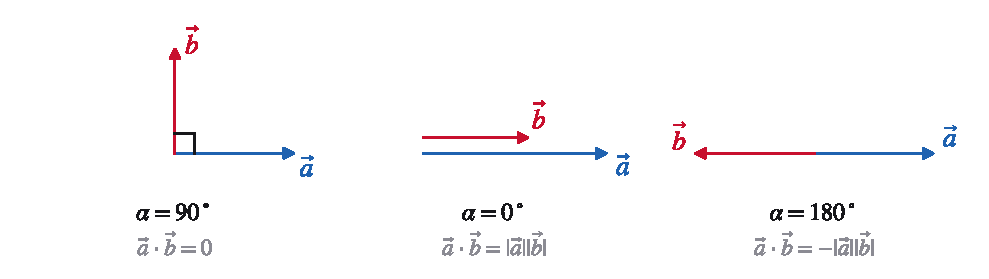
\includegraphics[width=372pt]{fig/m06_f15.pdf}
\caption{Interpretació geomètrica del producte escalar: perpendiculars ($\alpha = 90^\circ$), paral\textperiodcentered{}lels mateix sentit ($\alpha = 0^\circ$) i paral\textperiodcentered{}lels sentit contrari ($\alpha = 180^\circ$).}
\end{figure}

Les propietats geomètriques principals del producte escalar són:

\begin{enumerate}
\item \textbf{Angle entre dos vectors:}
\end{enumerate}

\begin{equation*}
\cos\alpha = \frac{\vec a\cdot\vec b}{|\vec a|\,|\vec b|} \;\Rightarrow\; \alpha = \arccos\!\left(\frac{\vec a\cdot\vec b}{|\vec a|\,|\vec b|}\right)
\end{equation*}

\begin{enumerate}
\item \textbf{Vectors perpendiculars o ortogonals:} $\vec a \perp \vec b$ si i només si $\vec a\cdot\vec b = 0$.
\end{enumerate}
